\documentclass[preprint]{aastex62}
\usepackage{graphicx}
\usepackage{amsmath}
\usepackage{natbib}
%\usepackage{subcaption}
\bibliographystyle{aasjournal}
\usepackage[version=4]{mhchem}

\begin{document}

\title{Expanding the Modeling of Type Ia Supernovae}
\author{Abigail Bishop}
%\date{}							% Activate to display a given date or no date

% General Guidelines
  % Write it like a scientific paper
  % Every sentence is precise and meaninful
  % Write with good English
  % UNDERSTAND the analysis and make that clear
  % Contain all information necessary to reproduce my analysis and results
  % Be concise
  % If you find yourself repeating sentences, consider making a table
  % Make sure there's a red thread
  
  % Figures
    % Ensure they're legible when printed out
    % Contain information 
    % Make sure the figure caption describes the figure adaquately
    % Make sure your results are reported in the body of the text, not just shown in a figure

\begin{abstract}
  % The abstract contains a summary of the paper.
  % A brief description of your observations
  % Your results!
  % Gets the point across
  % Good understanding of the subject and of your results
  % NOT lengthy introduction to the problem. No sentences like 'the aim was to learn about CCDs'. No information not in the main body of the paper
  
  Type Ia Supernovae are some of the most important astronomical events in the universe as they serve as standard candles that observational astronomers can use to make distance calculations and are the production mechanism for half of the iron in our universe. There are three main models of Type Ia supernovae, which include white dwarf mergers, sub-Chandrasekhar double detonations, and Chandrasekhar mass single detonations. A recent paper by Shen and Bildsten reveals that the simulations about the double detonation model, which make these supernovae so valuable, are not fully developed and may be leading to inaccuracies in measurements. This report details the process by which nuclear astrophysics codes like Pynucastro, Microphysics, and Castro are used to test the claims of Shen and Bildsten by simulating Type Ia Supernovae using the sub-Chandrasekhar double detonation model. Currently, it is clear that the initial detonation is propagating through the helium layer of a sub-Chandrasekhar mass WD. As the simulation continues to progress, we hope to see the second detonation then to move on to higher level simulations.

\end{abstract}

\pagebreak

\section{Introduction}

  % Serves as a review of the subject of the paper
  % Needs to discuss and cite the appropriate literature 
  % Good understanding of the subject and of your results

  Supernovae (SNe), the explosive deaths of stars, are some of the most spectacular events in the universe. A SNe occurs due to a thermonuclear explosion or a gravitational collapse. The Type Ia Supernovae is a thermonuclear SNe especially notable for its use as an astronomical measure of distance and for being the generator of one half of the iron in the universe \citep{ironhalfuniverse}. Type Ia supernovae occur when two stars are in orbit around each other where at least one star has already died once and has become a white dwarf (WD), usually with a mass around that of our sun ($M_{\odot}$). The close orbit leads to major gravitational interaction causing some material in the outer shells of the WD's partner to be transferred to the WD through its gravitational field. In the long-standing theoretical model, once the WD has taken enough material to reach a mass of 1.4 times $M_{\odot}$, it explodes. This 1.4$M_{\odot}$ is called the Chandrasekhar mass and is the greatest mass a white dwarf can have. The explosion releases enough energy to unbind the WD, expelling energy in the form of kinetic energy and light in many colors and other wavelengths. The graph plotting how bright each wavelength of light is in the explosion is the spectrum. Since these stars usually have the same mass and elemental composition when they explode, the explosions have the same brightness and uniquely Type Ia SNe spectrum characterized by a lack of Hydrogen and an abundance of Silicon \citep{SNeSpectra}. 
  
  An observational astronomer can observe an event resembling a Type Ia SNe and use its spectrum to confirm it is a Type Ia SNe. The astronomer can then take the brightness of the explosion and use it to calculate how far away the supernovae is. Type Ia SNe are called standard candles because the brightness of Type Ia SNe is consistent due to their fairly regulated mass. By using the observed brightness of Type Ia SNe in other galaxies to measure how far away they are, along with other measurements, observational cosmologists have been able to measure the rate at which our universe is expanding and note that the expansion rate is accelerating \citep{acceleratingUniverse1, acceleratingUniverse2}. We believe that an accurate understanding of Type Ia SNe is necessary to improve the precision of their use as standard candles. 
  
  The dilemma is that observational astronomers do not see as many Chandrasekhar mass WDs that could be involved in Type Ia SNe; however they see a lot of WDs in the sub-Chandra range where their mass is less than 1.4$M_{\odot}$. For this reason, astronomers are considering other explosion mechanisms based on the populations of WDs that they do observe. We intend to model the sub-Chandra WDs with the double-detonation model \citep{doubledet1, doubledet2}. Out of an increase in temperature, reactions in the Helium shell of a WD propel a shock wave through the WD's shell that compressed the core of the WD causing a second detonation. This difference in the explosion mechanism means the overall brightness and the spectrum of the explosion is slightly different from the Chandrasekhar mass Type Ia Supernovae. We hope that by modeling Type Ia SNe in this fashion, they will match with observations. This has been done before, however, the paper \citet{shenNbildsten} has pointed out that previous simulations have not included as many possible nuclear reactions as it should have to make the calculations accurate. In this thesis I discuss the methods by which we use a computer code to simulate Type Ia SNe with the nuclei and reactions suggested by Shen and Bildsten. 

\section{Codes}
  	
    We use several codes developed by our group, all of which are available on GitHub. GitHub is a website used to mediate code sharing and code collaboration. Most of the codes discussed in this report available for viewing, editing, and using (also known as open-sourced software). This helps to promote reproducibility and encourages community contributions to the projects. 
    %Maybe a little more here if I can finesse it.

  \subsection{Pynucastro}
    
    Pynucastro\footnote{\url{https://github.com/pynucastro/pynucastro}} is an open-sourced coding package developed by Dr. Michael Zingale and Dr. Donald Willcox to create networks of nuclear reactions that can be used in their simulations \citep{pynucastro}. It does so by collecting information on the rate at which nuclear reactions occur at different temperatures from a database called the JINA Reaclib Database \citep{JINA}. Using the Pynucastro Python library, a script can be written that will incorporate specifically chosen JINA reaction rates into a model and rates that can be used in Microphysics and Castro simulations.
  
  \subsection{Microphysics}
  
    Microphysics\footnote{\url{https://github.com/starkiller-astro/Microphysics}} is an open-sourced software that I have been a core contributor to which has routines designed to incorporate aforementioned networks of reaction rates into astrophysical simulations \citep{Microphysics}. This is done through the solving of ordinary differential equations for updated abundances resulting from the burning. It is equipped with unit tests designed to run stellar simulations in a short amount of time to troubleshoot problems on a small scale before promoting the simulations to a larger scale operation. Microphysics comes with some preexisting networks but can also use new networks generated by Pynucastro. 
  
  \newpage
  
  \subsection{Castro}
  
    Castro\footnote{\url{https://github.com/AMReX-Astro/Castro}} is an open sourced hydrodynamics code designed to run full scale simulations of astrophysical events in one dimension, two dimensions, and three dimensions \citep{castro}. Castro is initialized with a model that includes a stellar object and information about its density, temperature, and pressure. This code solves equations for conservation of total mass, momentum, energy, other hydrodynamics equations, and Poisson's equation for self-gravity together with the equation of state. The effects of burning are coupled in using a Strang Splitting technique \citep{strang} to calculate the evolution of the initial model over time. All of these equations need to be solved for individual points on a line (for 1-Dimensional simulations), in a grid (2-D), or in a box (3-D) which is very time and computationally expensive. Adaptive Mesh Refinement (AMR) is used to assist with this as it will request that fewer zones be solved in regions of the simulation where there is less activity but will also request that more zones be solved in very exciting regions leading to a more resolved and accurate picture. To further help with the computationally expensive nature of this process, Castro has been designed to run on supercomputers that can drastically cut the run time of these simulations. To date, Castro has been used to conduct many exciting simulations like Type Ia SNe \citep{subch1, subch2}, core collapse SNe \citep{corecollapse1, corecollapse2}, and WD mergers \citep{merger}. 
  
\section{Motivation}
  
  As previously mentioned, Type Ia SNe are critical to measuring large astronomical distances. In the paper \citet{shenNbildsten}, it is theorized that additional reactions are required to accurately simulate the early part of helium burning in Type Ia supernovae. Additionally, not all Type Ia SNe occur when the WD becomes a total of 1.4 $M_{\odot}$. In the double detonation model, Type Ia supernovae can occur in the sub-Chandrasekhar regime because a hot spot in the Helium layer of a WD causes a thermonuclear reaction runaway sending a shockwave through the Helium layer. This shock wave hits the Carbon-Oxygen core of the WD and initiates the Type Ia. Being sub-Chandrasekhar means that these SNe could have different observational signatures that Chandrasekhar mass Type Ia SNe. It is critical that accurate models of Type Ia SNe are obtained in order for observational astronomers to learn about the universe accurately. 
  
  The goal for this research is to first create a nuclear reaction network following Shen and Bildsten's guidelines, test the network in Microphysics to see if there is a substantial change, then to run a model without the elements and reactions suggested by Shen \& Bildsten to be compared with a model that does consider their recommendations. If the change in results is drastic, then we will have sufficient motivation to conduct more detailed calculations to understand these consequences. 
  
\section{Simulations and Results}
  
  \subsection{Pynucastro}
    
    {\tt Aprox13} is a nuclear reaction network composed of 13 isotopes \citep{timmes}. It begins with Helium (\ce{^4He}, also known as an $\alpha$ particle) adds two $\alpha$ particles to get a Carbon (\ce{^{12}C}) and one photon ($\gamma$) then continues to add $\alpha$ particles until Iron (\ce{^{56}Fe}) and a lot more $\gamma$'s are obtained. Since each isotope is connected by an $\alpha$ particle, this is called an $\alpha$ chain and earns the name 13 from the 13 isotopes on the $\alpha$ chain that it possesses. All elements that are \ce{^{24}Mg} and heavier are also connected through a process where an $\alpha$ particle hits an isotope and creates a new particle but kicks out a proton, then a different proton hits the new nucleus and one of those $\alpha$ chain isotopes are created along with a $\gamma$. In total the {\tt aprox13} network contains 13 isotopes and has proven to be a good model of stellar evolution, but \citet{shenNbildsten} suggests adding additional rates to the beginning of this double-detonation model for Type IaSNe.  
    
    This study began through the use of Pynucastro to create the {\tt subch} network, standing for sub-Chandrasekhar. The network is composed of 8 reactions and 11 isotopes, with Nuclear Equations  \ref{chemeq:1.1}, \ref{chemeq:1.2}, \ref{chemeq:2.1}, \ref{chemeq:2.2}, and \ref{chemeq:3.2} being the ones suggested by \citet{shenNbildsten} and the remaining three being a part of the $\alpha$ chain processes. The big change made through the generation of this network is the addition of \ce{^{14}C} and \ce{^{14}N} which will be the key players in expediting the explosion in this model. A visual diagram of the reactions in the {\tt subch} network is shown in Figure~\ref{fig:network}.
        
    \begin{align}
            \ce{3 ^4He &->  ^{12}C + 2\gamma } \\ 
            \ce{^{12}C + ^4He &->  ^{16}O + \gamma } \\
            \ce{^{14}N + ^4He &->  ^{18}F + \gamma } \label{chemeq:1.1} \\
            \ce{^{18}F + ^4He &-> ^{21}Ne +  p+} \label{chemeq:1.2} \\
            \ce{^{12}C + p+ &-> ^{13}N + \gamma } \label{chemeq:2.1} \\
            \ce{^{13}N + ^4He &-> ^{16}O + \text{p}} \label{chemeq:2.2} \\ 
            \ce{^{16}O + ^4He &-> ^{20}Ne + \gamma } \\
            \ce{^{14}C + ^4He &-> ^{18}O + \gamma } \label{chemeq:3.2}
    \end{align}
    
    \begin{figure}
      \centering
      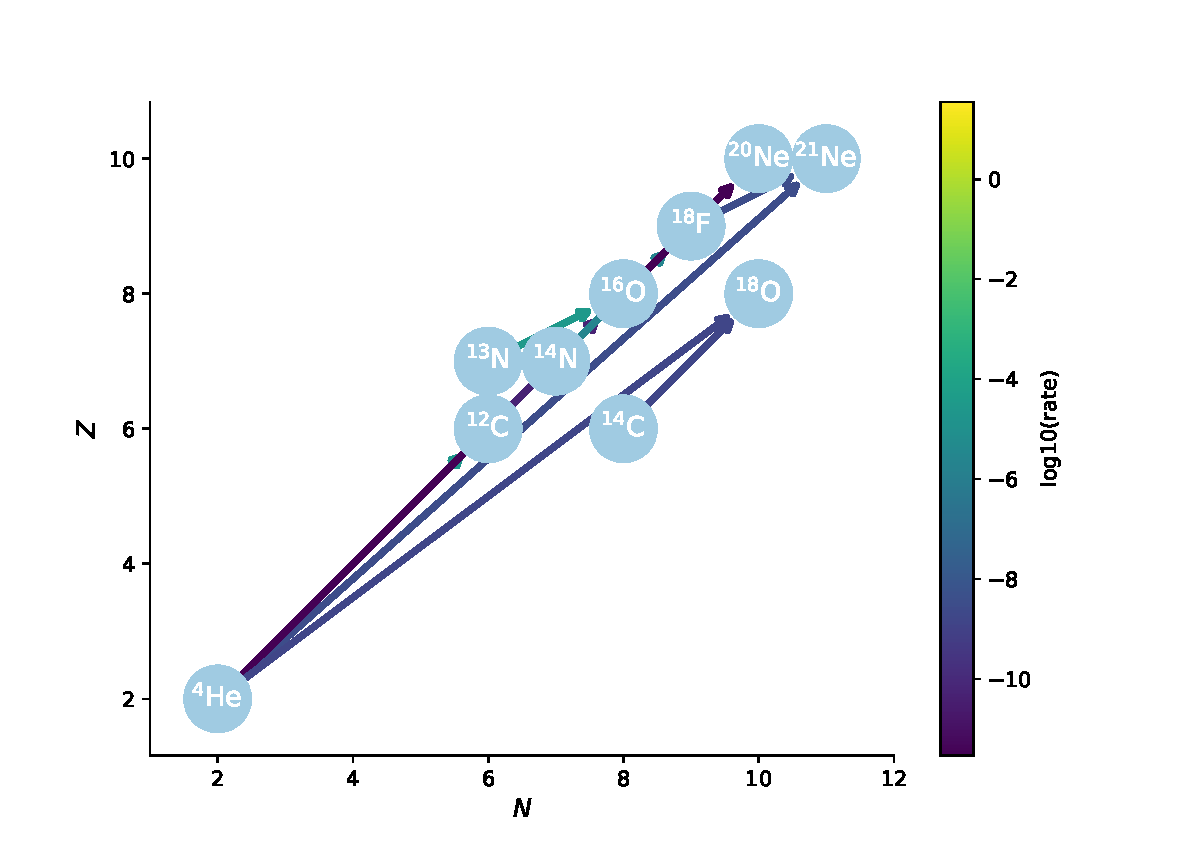
\includegraphics[width=5in]{images/subch}
      \caption{The {\tt subch} network reactions shown by connecting the isotopes involved on a plot of proton number ($Z$) by neutron number ($N$). Interactions with higher rates (yellow-green arrows) tend to occur more quickly than the slower interactions (blue-purple arrows).}
      \label{fig:network}
    \end{figure}
  
  \subsection{Microphysics}
  
    This new network is now used in Microphysics. There is a unit test in Microphysics referred to as {\tt burn\_cell} which simulates the chemical evolution in one small zone of a star. This test is first used to determine what tolerance will optimize results and reduce computation time in this simulation. Using these results, the {\tt burn\_cell} test will be used to simulate the chemical evolution of this zone as nuclear reactions take place to use and generate different elemental isotopes. 
  
    \subsubsection{Testing Simulation Equation Tolerances}
  
      Tolerances are parameters used to gauge how hard the ordinary differential equation solvers in the simulation must work. Smaller tolerances lead to many smaller steps which is more work for the solves. These equations are all coupled and integrated numerically, so a good accuracy is critical. A smaller tolerance typically leads to a more precise answer but takes more computer time. For this reason, a tolerance of $10^{-12}$ was treated as an exact answer since it is very small but still significantly more than round off error ($10^{-16}$). The tolerances of $10^{-3}$, $10^{-6}$, and $10^{-9}$ were tested with respect to the test with a tolerance of $10^{-12}$. 
     
      To test these tolerances, \ce{^4He} was initialized in one zone as modeled by the {\tt burn\_cell} unit test. The zone is heated so that the \ce{^4He} begins to burn into \ce{^{12}C} and \ce{^{16}O}. Simulations are run with a tolerance of $10^{-3}$, $10^{-6}$, $10^{-9}$, and $10^{-12}$ in a zone that is initialized to a temperature of $T = 3 \times 10^8$ K and a density of $\rho = 1 \times 10^6$ g/cm$^3$. The relative error in each element's mass fraction, $X$, is calculated between the 3 simulations with looser tolerances and the $10^{-12}$ simulation, as defined by 
    
      \begin{equation}
        \sigma_X = \frac{\lvert X_{10^{-12}} - X_{\text{former}} \rvert }{X_{10^{-12}}} \text{    , }
        \label{eq:relativeerror}
      \end{equation}
    
      \noindent for each point in time during the simulation. This relative error in mass fraction is plotted as a function of time for each of the three testing simulations and can be seen in Figure~\ref{fig:relativeerror}.
    
      \begin{figure}
        \centering
        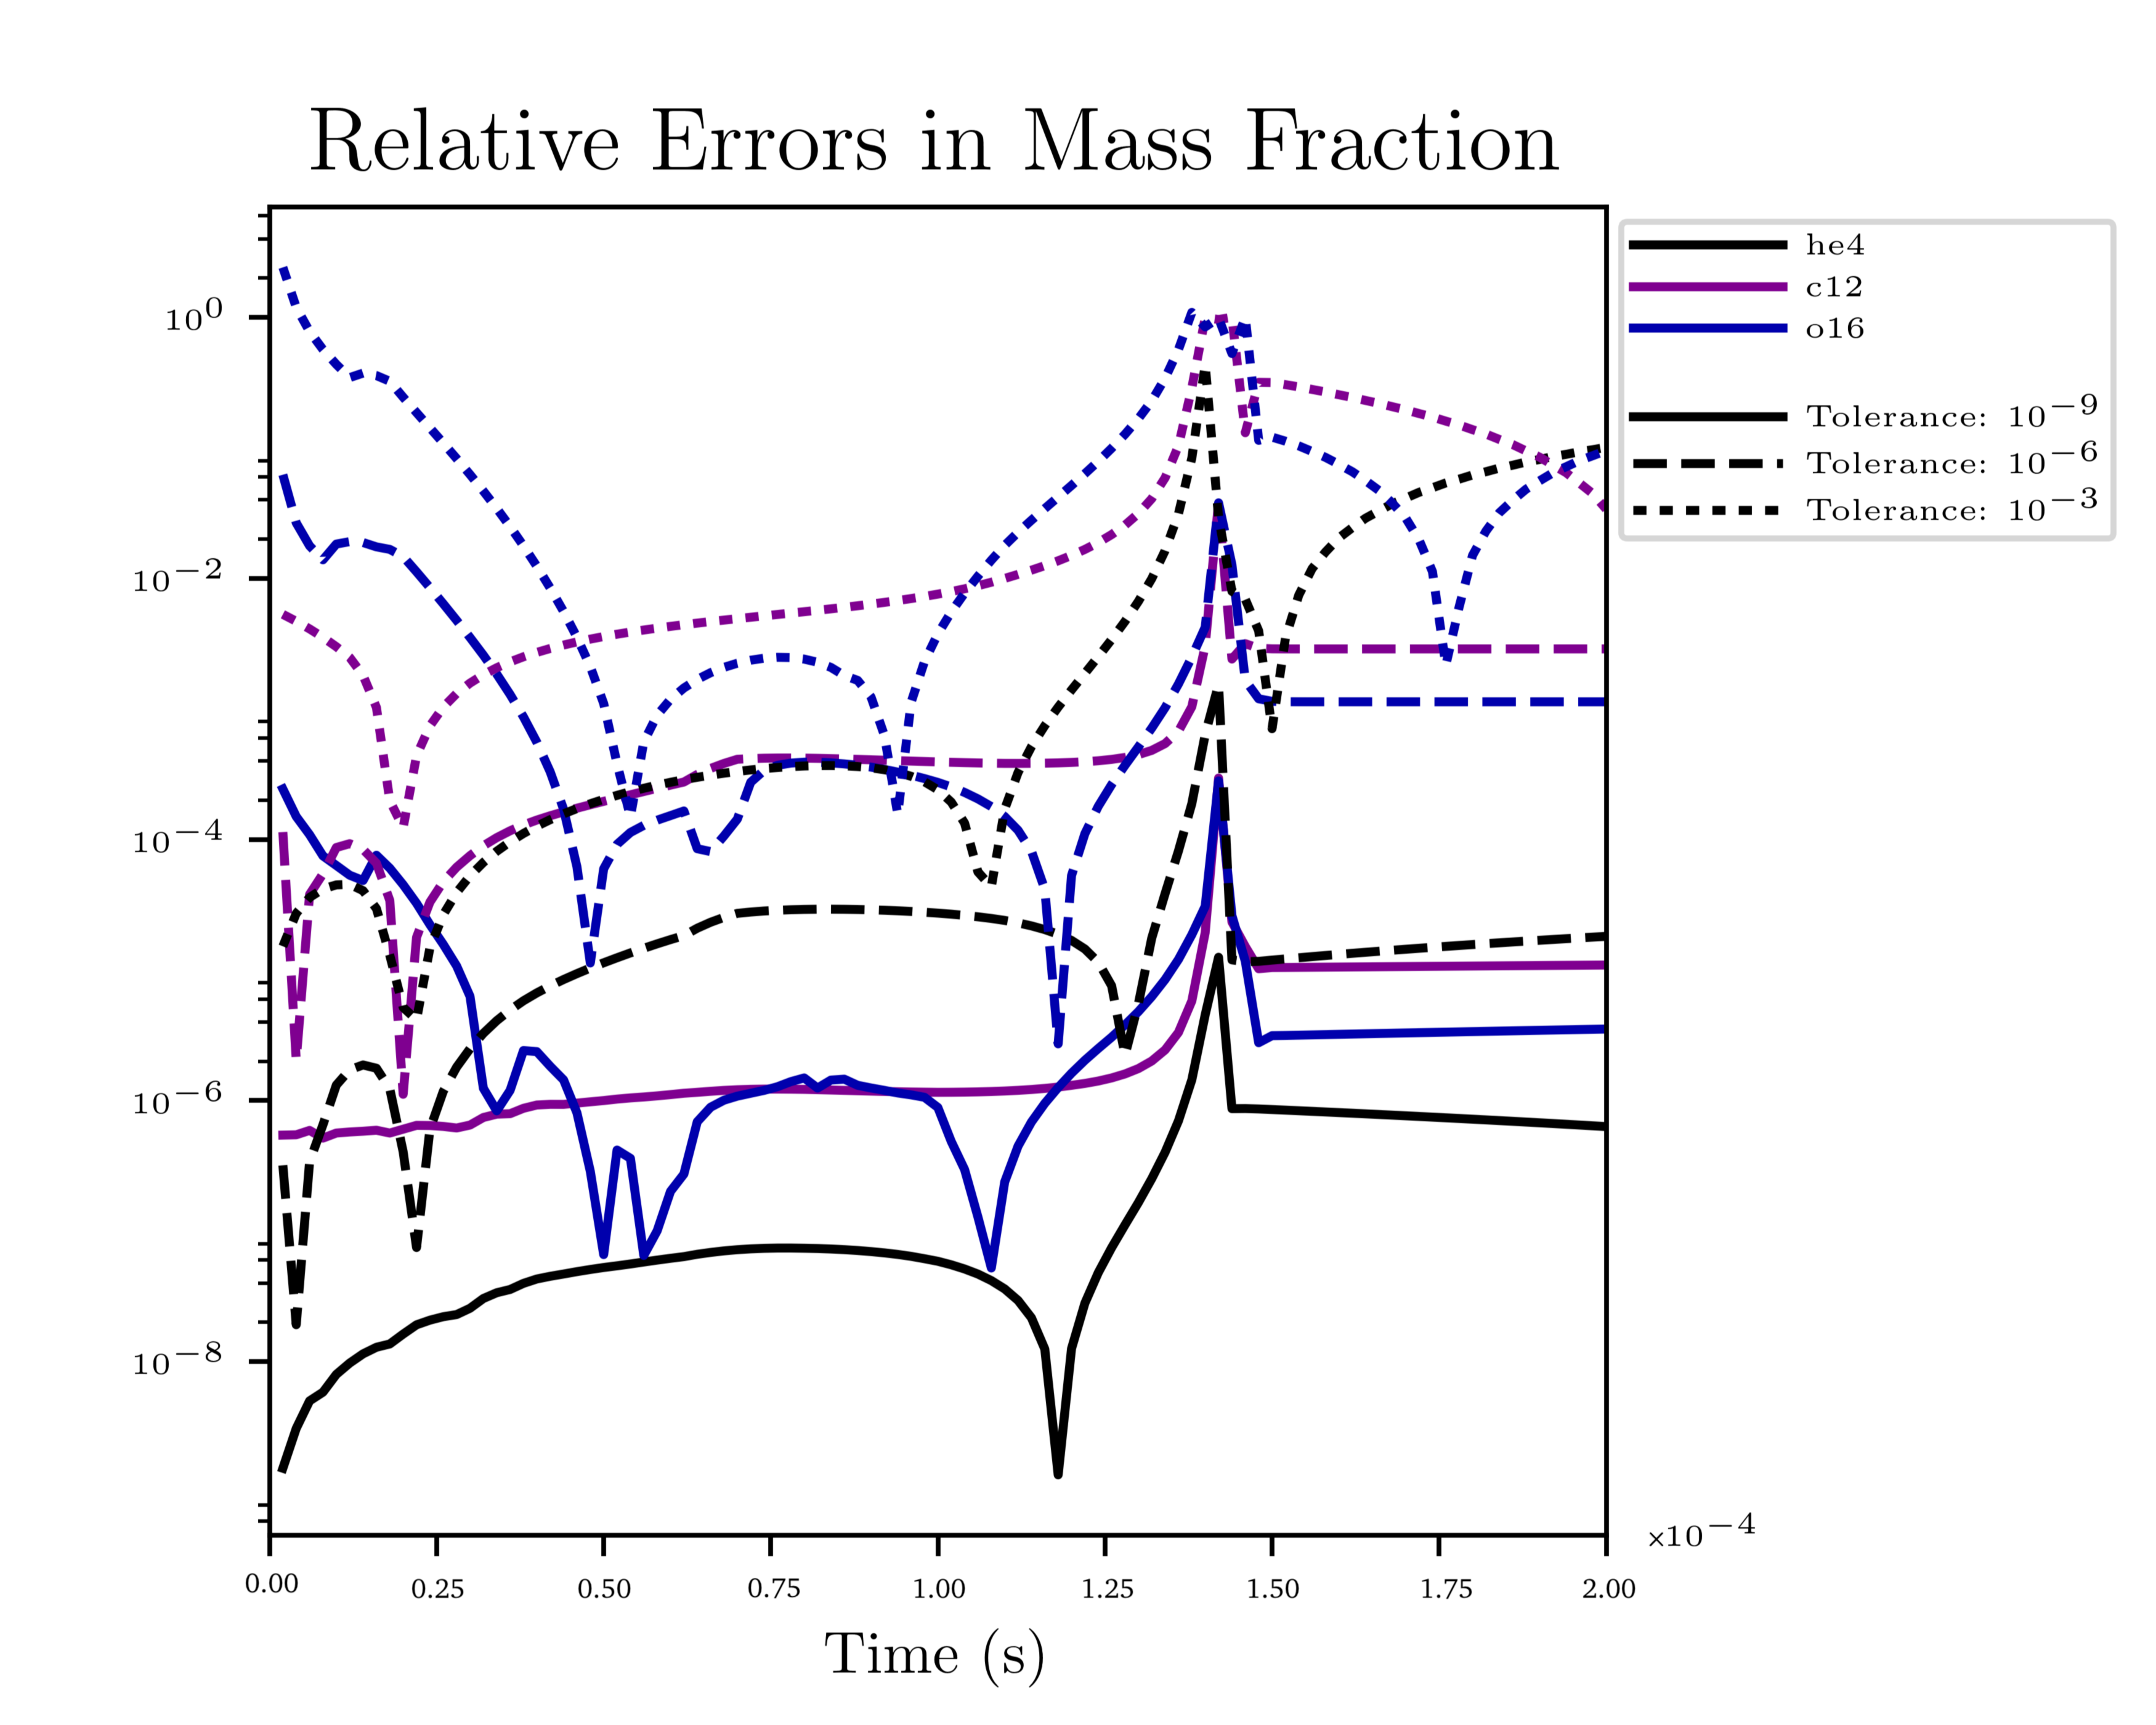
\includegraphics[width=5in]{images/react_aprox13_test13_ureca_tol-rel_xn1.png}
        \caption{Relative error over time of the \ce{^4H} (in black), \ce{^{12}C} (in purple), and \ce{^{16}O} (in blue) mass fractions run in simulations with a tolerance of $10^{-9}$ (solid line), $10^{-6}$ (dashed line), and $10^{-3}$ (dotted line) calculated with respect to the true values calculated by a simulation with a tolerance of $10^{-12}$. The lower the value, the closer the result is to the true value.
          }
        \label{fig:relativeerror}
      \end{figure}  
  
      From Figure~\ref{fig:relativeerror}, one can see that the solid lines, corresponding with the simulation using a tolerance of $10^{-9}$, are consistently the lowest. The relative error of the simulation with a tolerance of $10^{-9}$ is consistently below $10^{-3}$ and drops as low as $10^{-8}$ at times without taking much longer to run than the simulations with tolerances of $10^{-6}$ and $10^{-3}$. Therefore, we believe that a tolerance of $10^{-9}$ yields an acceptable amount of error for our simulations.
  
    \subsubsection{Using Mass Fraction Evolution to Justify Motivation}
    
      The next step with the {\tt burn\_cell} tests is to test if the {\tt subch} network is producing results worth investigating. The main ingredients to the simulation that Shen \& Bildsten encouraged were \ce{^{14}C} and \ce{^{14}N} \citep{shenNbildsten}. Figure~\ref{fig:microphysicsX} shows the time evolution of mass fractions, $X$, for each of the eleven isotopes in the {\tt subch} network for three different {\tt burn\_cell} simulations. This zone, too, is initialized at $T = 3 \times 10^8$ K and $\rho = 1 \times 10^6$ g/cm$^3$. One simulation is run without \ce{^{14}C} and \ce{^{14}N}, one with some \ce{^{14}N}, and the last with both \ce{^{14}C} and \ce{^{14}N}. If Shen \& Bildsten's theory is correct, we shouldn't see the dashed and dotted lines overlay the solid lines, but dashed and dotted lines following different paths and implying that there is a notable change in each of the simulations. In Figure~\ref{fig:microphysicsX}, seeing a combination of solid, dashed, and dotted lines at different orders of magnitudes for many elements implies that the incorporation of \ce{^{14}C} and \ce{^{14}O} is important. 
      
      \begin{figure}
        \centering
        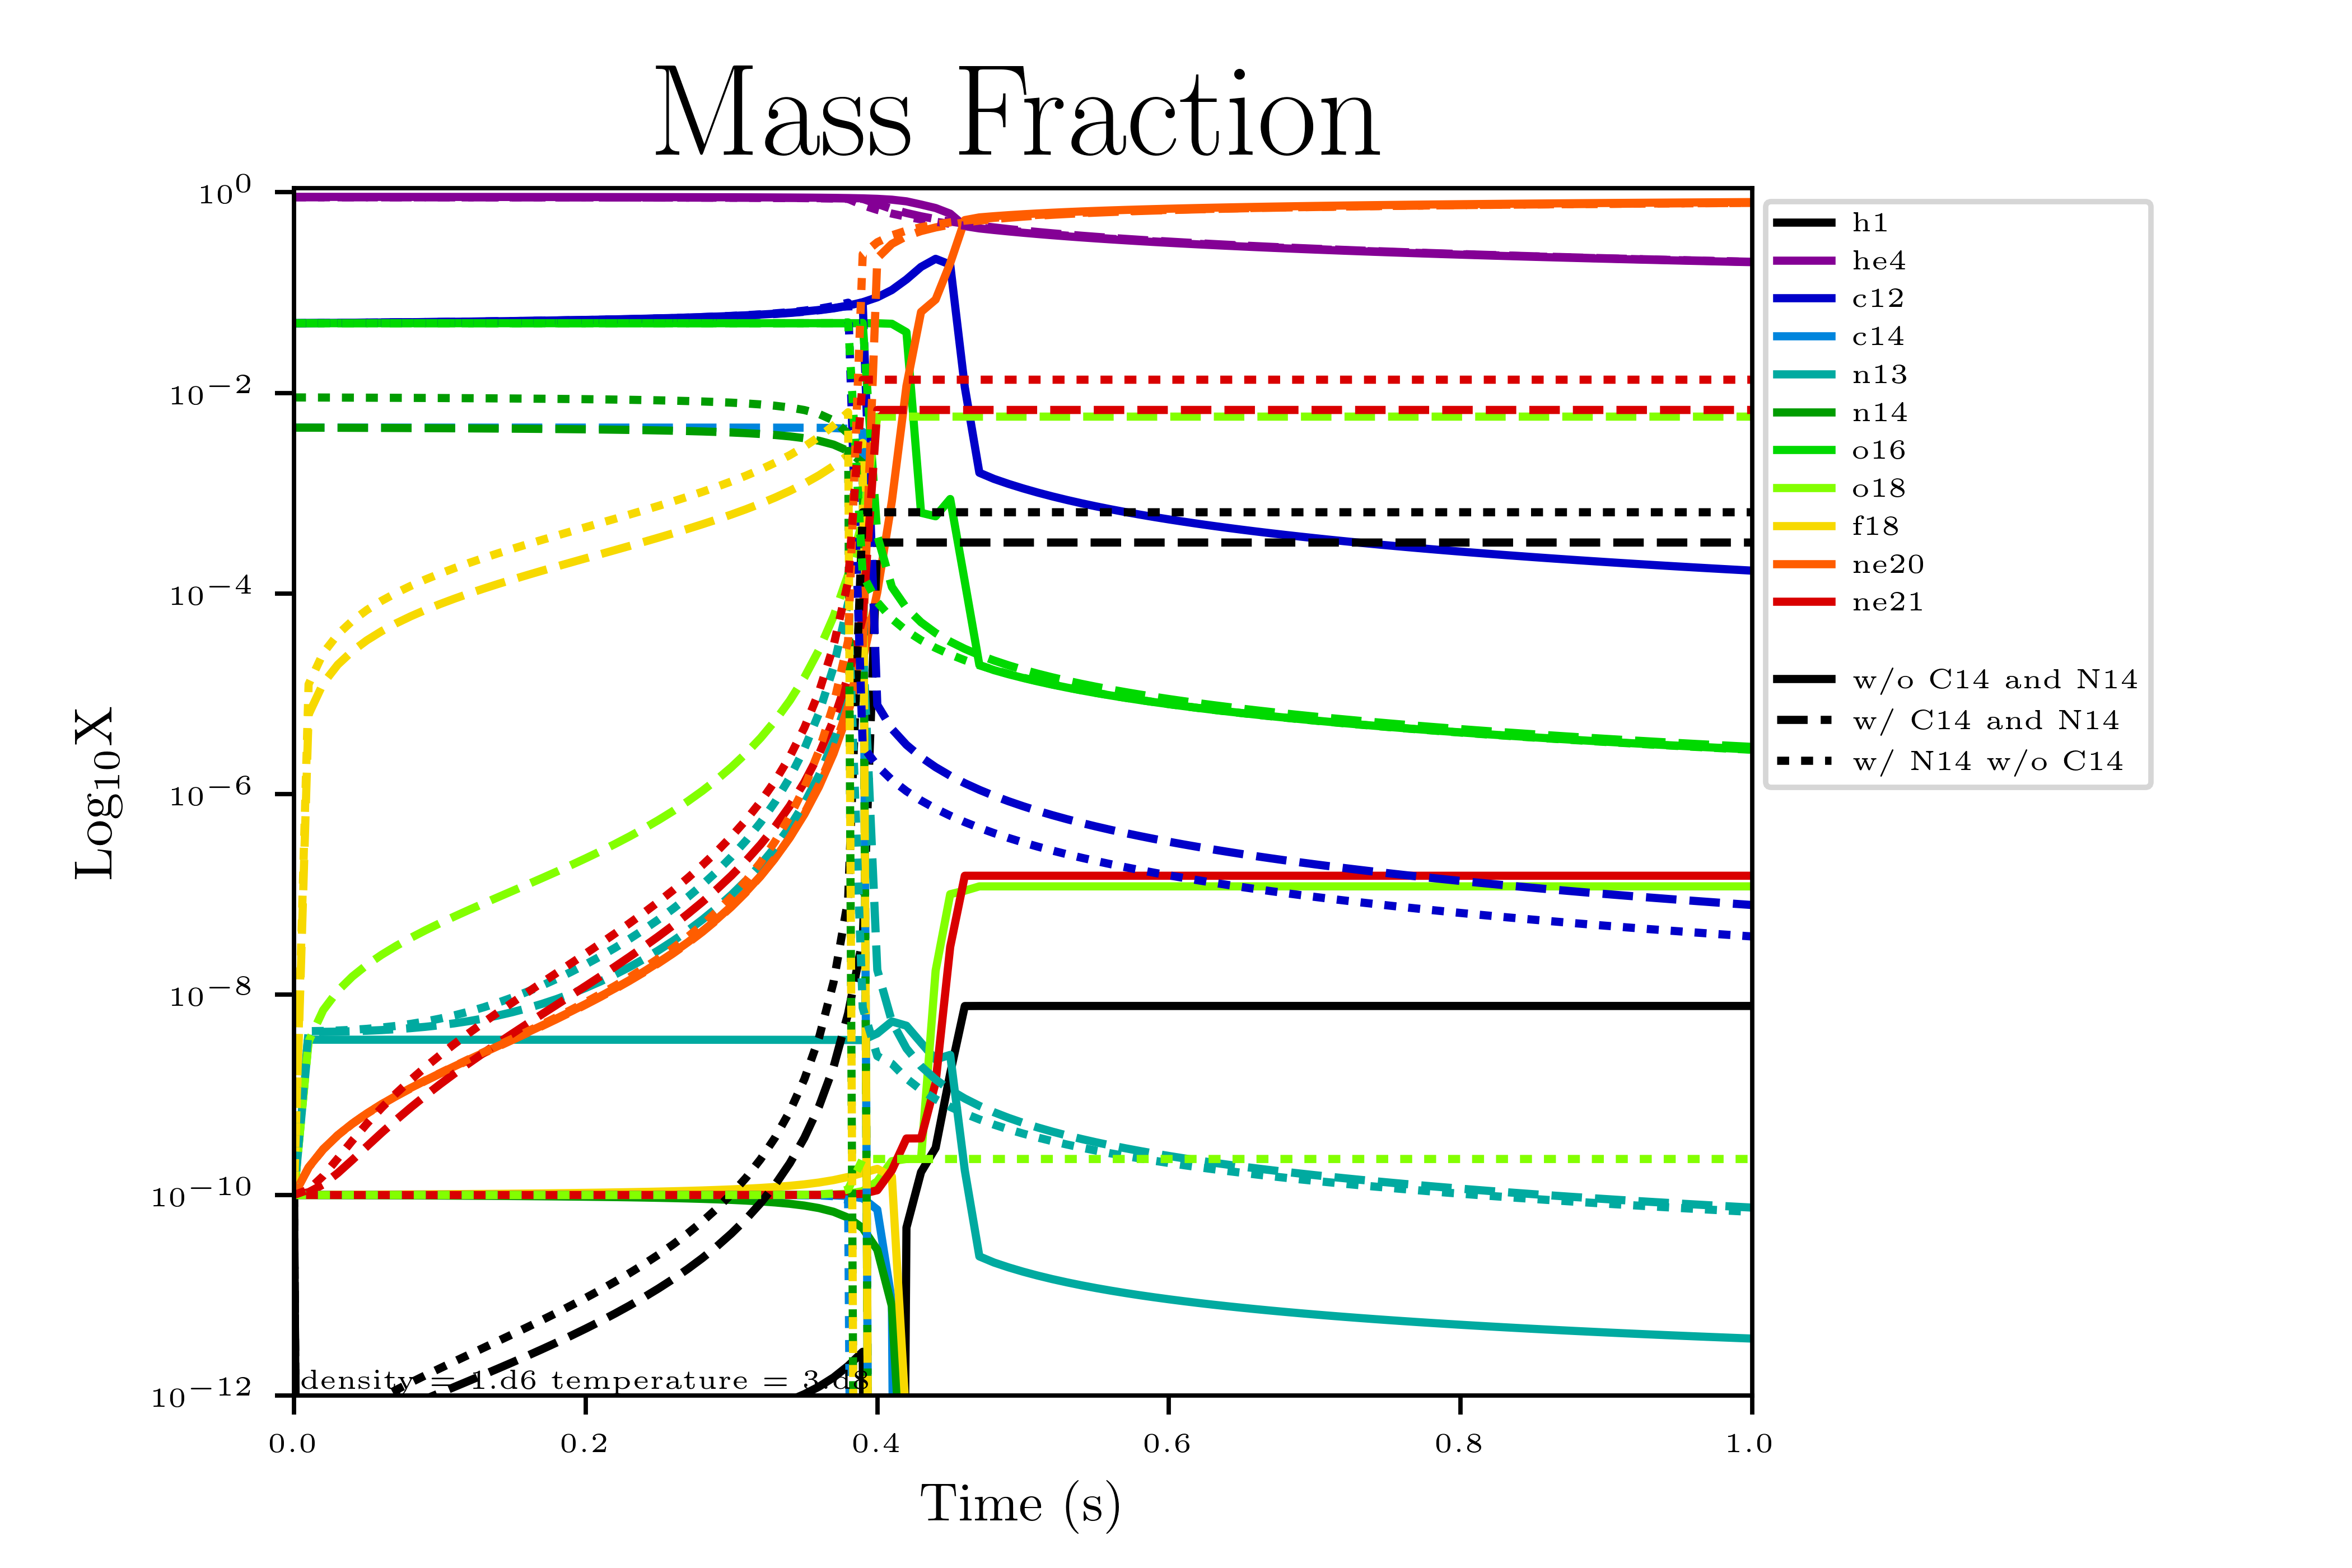
\includegraphics[width=5.5in]{images/subch_nC14nN14_xn_tol-10.png}
        \caption{Mass fraction, $X$, evolution over time for the 11 elements (differentiated by color) in the {\tt subch} network for three different {\tt burn\_cell} simulations: one without \ce{^{14}C} and \ce{^{14}O} (solid lines), one with both \ce{^{14}C} and \ce{^{14}O} (dashed line), and with \ce{^{14}O} but no \ce{^{14}C} (dotted line). Notice the large change in \ce{^{12}} and \ce{^{21}} between the simulations.
          }
        \label{fig:microphysicsX}
      \end{figure} 
      
      In addition to the mass fraction evolution, the rate of energy generated by the zone in the {\tt burn\_cell} simulation is plotted as a function of time in Figure~\ref{fig:energygeneration}. Once more, this is done for a simulation without \ce{^{14}C} and \ce{^{14}N}, adding only \ce{^{14}N}, and adding both \ce{^{14}C} and \ce{^{14}N}. From Figure~\ref{fig:energygeneration} one can see that in the simulations with \ce{^{14}C} and \ce{^{14}N}, the energy generated by this zone peaks sooner and has a lower peak.  This shows that when \ce{^{14}C} and \ce{^{14}O} are incorporated into the simulations of Type Ia SNe, they will generate energy faster, release their nuclear potential energy more quickly, and have a smaller maximum energy generation rate than simulations without these elements. This is another nudge in the direction of running a full-scale simulation. 
      
      \begin{figure}
        \centering
        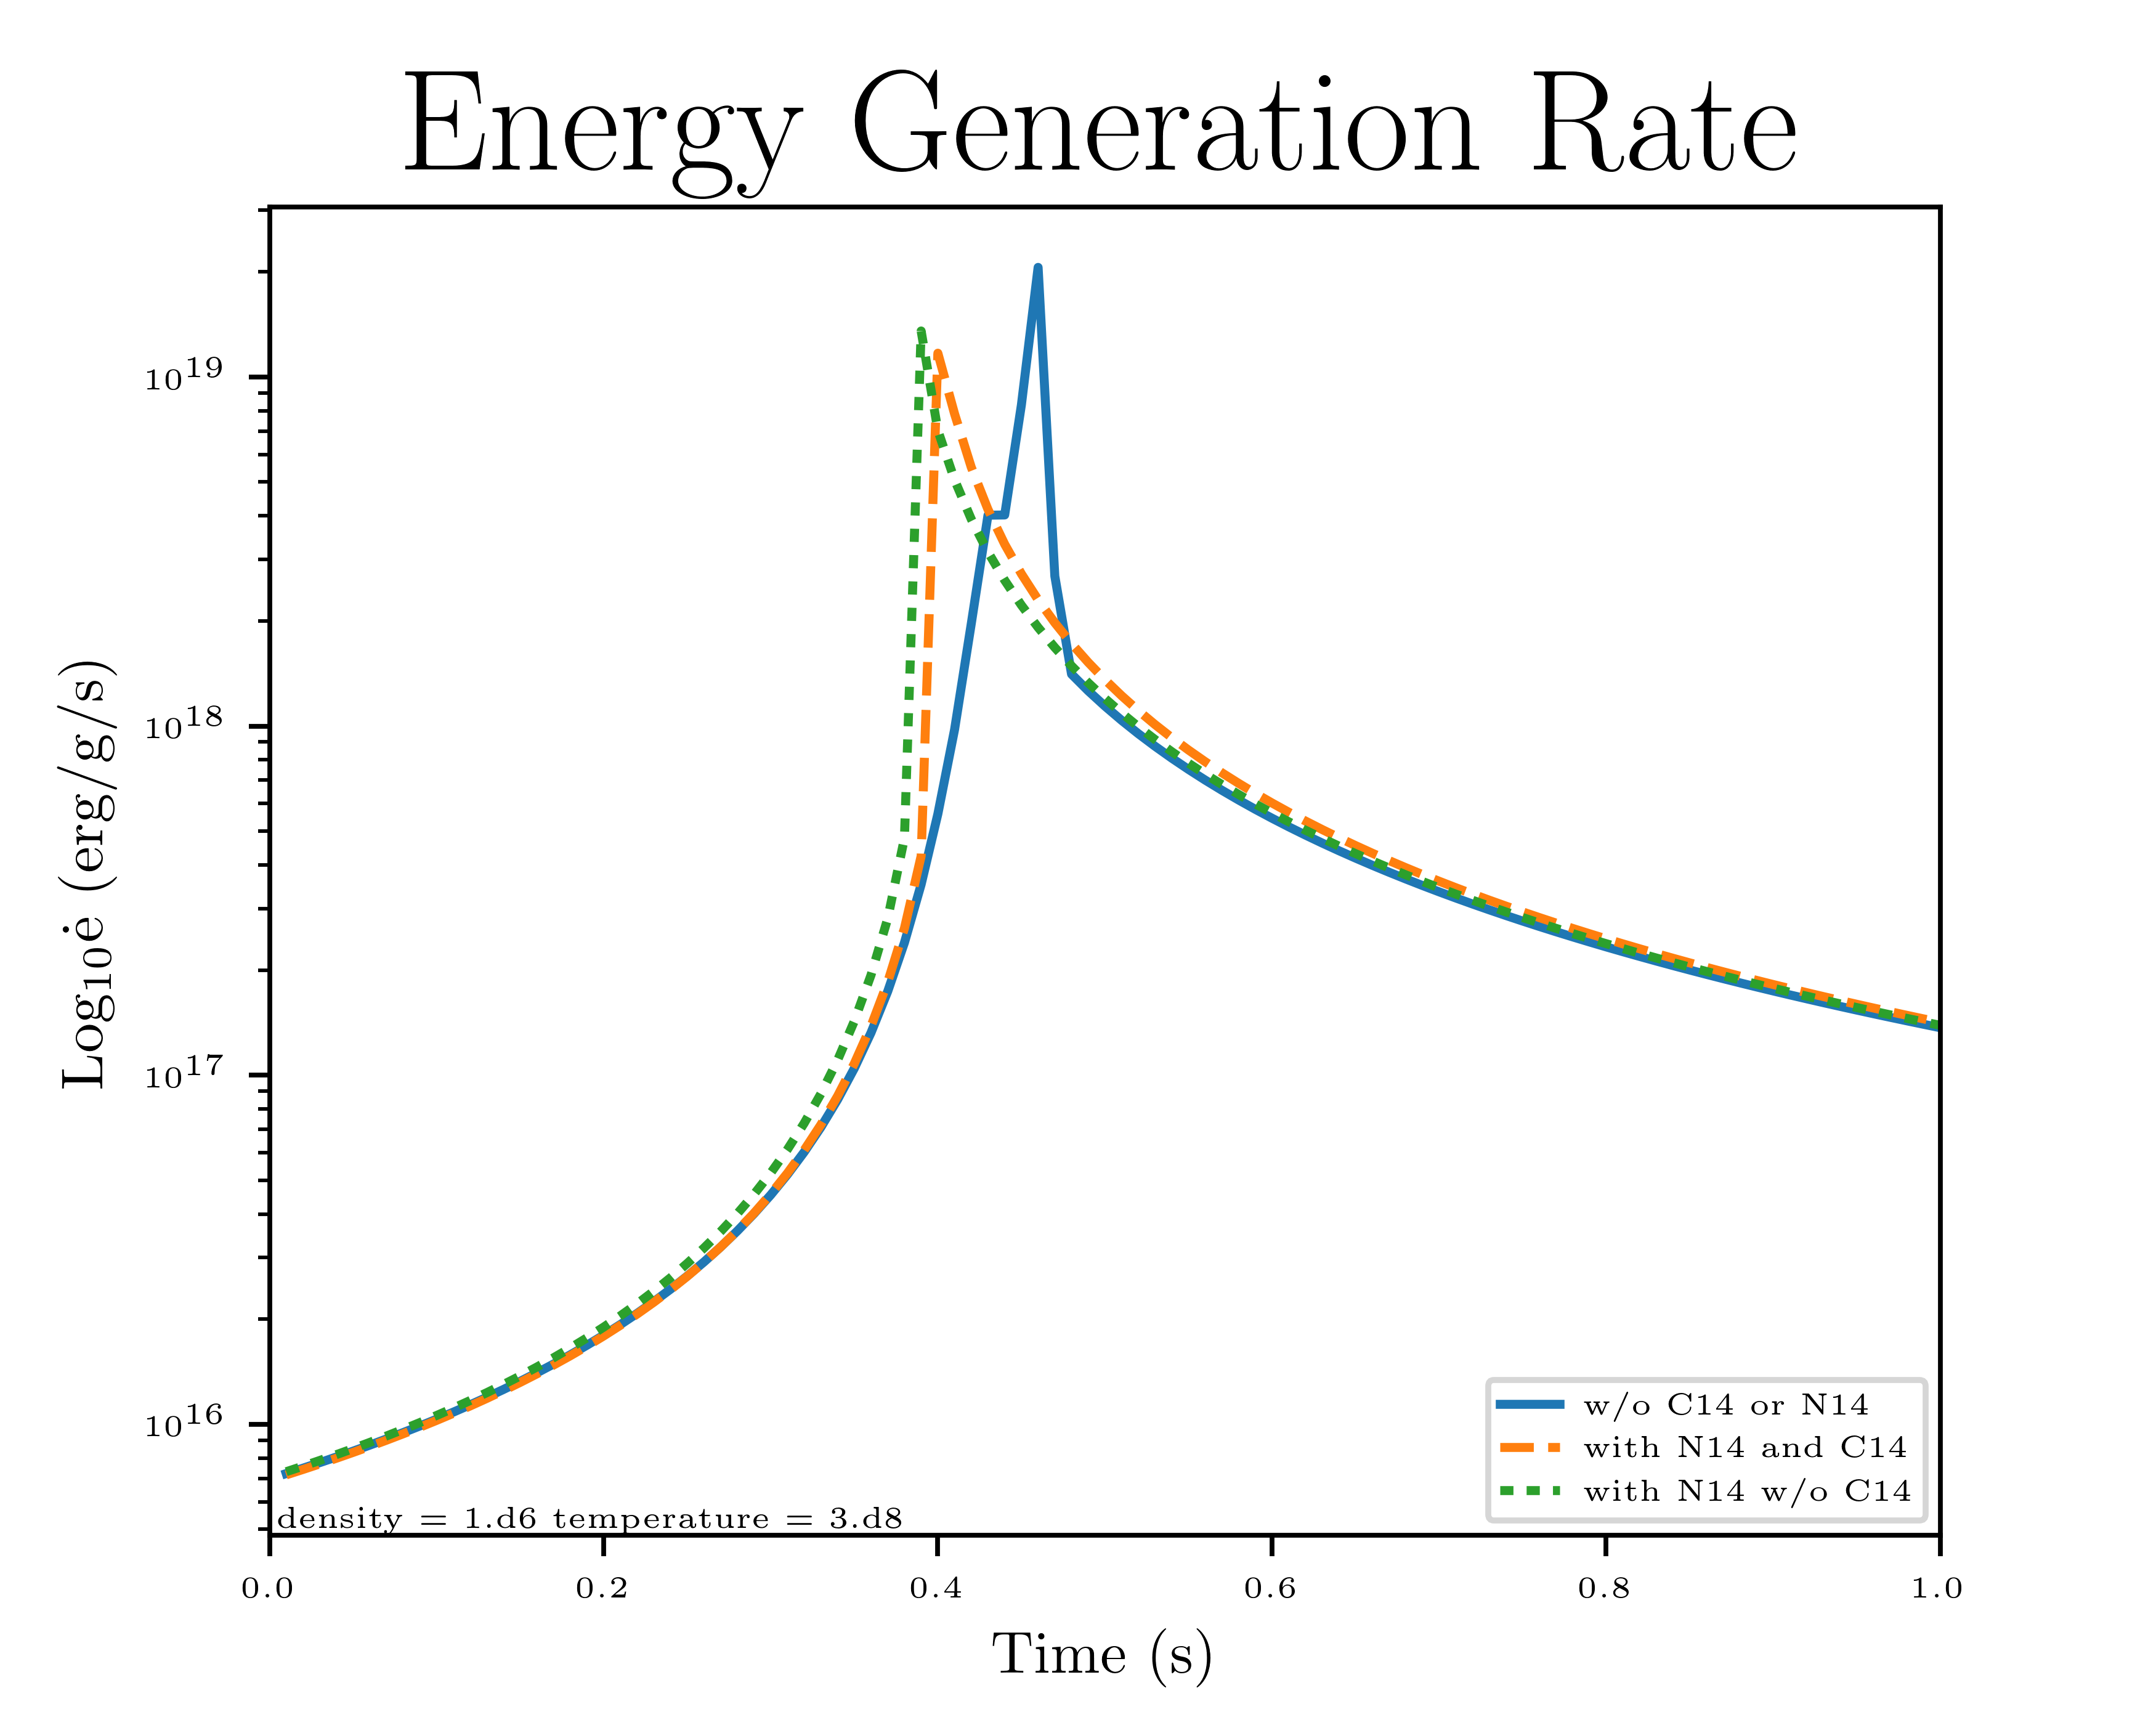
\includegraphics[width=4.5in]{images/subch_nC14nN14_edot_tol-10.png}
        \caption{The rate of energy generated by the zone in the {\tt burn\_cell} simulation as a function of time for the run without \ce{^{14}C} and \ce{^{14}O} (solid lines), with both \ce{^{14}C} and \ce{^{14}O} (dashed line), and with \ce{^{14}O} but no \ce{^{14}C} (dotted line).
          }
        \label{fig:energygeneration}
      \end{figure} 

  
  \subsection{Multi-dimensional simulations with Castro}
  
    The Castro code will be used to first test the {\tt subch} network in one dimension to see if an increase in temperature will ignite a detonation and push it across a layer of helium. A detonation occurs in a star when a thermonuclear runaway causes a supersonic shockwave to move through a medium, closely followed by a reaction zone. If a denotation occurs, then the Castro code will be used to simulate the star in two dimensions. This can then be compared to simulations of stars using other networks and the results can be compared. 
    
    \newpage
    
    \subsubsection{1-Dimensional Simulations}
    
      Using the Castro science problem called ``Detonation", a simulation of a shock wave propagating from left to right was initialized with the {\tt subch} network. The layer of helium that this wave is propagating through has a density of $\rho = 1 \time 10^6$ g/cm$^3$, has a shock wave with a temperature of $T = 2 \times 10^9$ K (on the left), and has a resting temperature of $T = 0.05 \times 10^9$ K (on the right). These inputs were selected to match the conditions we expect to see at the base of the helium layer in the sin-Chandrasekhar model. As shown in Figure~\ref{fig:detonation}, the energy released from nuclear reactions in the detonation powers a wave to the right side of the screen and off of the page. 
      
    \begin{figure}
      \centering
      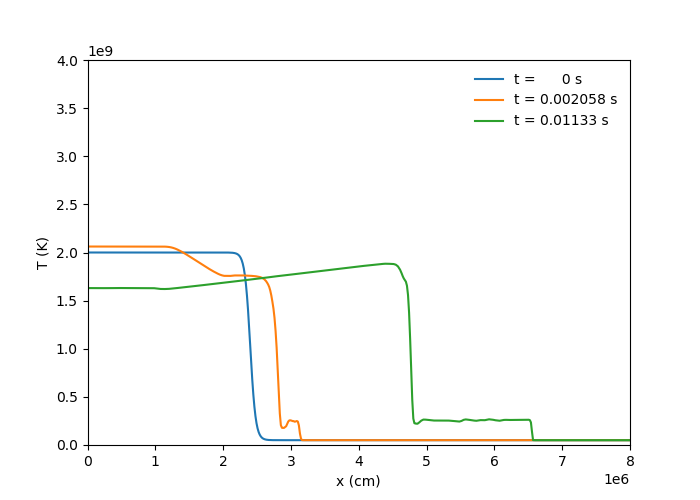
\includegraphics[width=5in]{images/flame-thesis}
      \caption{The above images depict a detonation wave (shown by a shelf of temperature on the left at 2 billion K) propagating in the right direction at the beginning of the simulation (Figure (a)), after 0.002 seconds (Figure (b)), and after 0.01 seconds (Figure (c)).}
      \label{fig:detonation}
    \end{figure}
      
      Now, knowing that a mild temperature perturbation can ignite a helium layer, this simulation can be taken to two dimensions, which is a big step. These one-dimensional simulations take a couple minutes to run on an average computer but the two dimensional simulations will take much longer, even on a much larger computer. 
        
    \subsubsection{2-Dimensional Simulations}
  
      The two-dimensional simulations are completed by wrapping a \ce{^{12}C} and \ce{^{16}O} WD core in a thick layer of \ce{^4He} and simulating it in axisymmetric coordinates. The burning is initiated by a hot temperature perturbation at the interface between the helium shell and the core along the north pole of the star. Figure~\ref{fig:subchsims} shows this setup. 
      
      \newpage
      
      The domain of simulation is $1.25 \times 10^9$ cm wide by $2.5 \times 10^9$ cm high, 3 levels of refinement are used (more levels, more accurate, longer run time), a perturbation temperature factor of 80, a perturbation radius factor of 8 (meaning a perturbation radius of $8 \times (2.5 \times 10^6) \text{ cm} = 2 \times 10^7 \text{ cm}$ or 200 km), centered at a distace of 0.35 billion centimeters from the center from the star. Using the {\tt subch} network to simulate this, the images in Figure~\ref{fig:subchsims} resulted. At the top of the star in the second image, it is clear that the shock wave is propagating across the helium layer of the WD and that the front of the shock wave has a temperature near $2.5 \times 10^9$ which is very high and very promising. 
      
      \begin{figure}
        \gridline{
          \fig{images/subch_20190505_plt00000_Temp_slice}{0.48\textwidth}{(a)}
          \fig{images/subch_20190505_plt95900_Temp_slice}{0.48\textwidth}{(b)}
          }
        \caption{These plots were created using {\tt amrvis} which can be found in the AMReX coding package \citep{AMREXcodes}. They depict the WD as a half circle in the left middle and use color to display the temperature in the plane. A redder color is a cooler temperature and a yellow color represents warmer temperatures. Note that the values associated with the color scale of the temperature may change between pictures. 
          }
        \label{fig:subchsims}
      \end{figure}

\newpage

\section{Conclusion}

  % Summary of the analysis
  % Emphasis is on the results and their interpretation, and how they relate to results in the literature
  % Can provide an outlook, e.g. how the measurement can be improved with future measurements
  % Good understanding of the subject and of your results
  
  Shen \& Bildsten's paper brought light that simulations of Type Ia SNe needed more work, motivating the investigation narrated in this report. After checking the accuracy of codes used, simulations using a network of nuclear reaction rates based off of the Shen \& Bildsten paper were used in a one zone simulation, moving to a one-dimensional simulation, and culminating in an insightful two-dimensional simulation \citep{shenNbildsten}. I had a central role in debugging a series of issues with the code, from posting and working through a GitHub Issue, to interacting with the developers of the Castro code, to running many tests to resolve the issue. After a few months of struggling with and manipulating the Castro code and inputs values, we reminded ourselves of the importance of setting accurate lower limits for qualities such as density and reminding the code to reevaluate the adaptive mesh refinement gridding frequently. Now that the simulation is running, it is shown that the shock wave will propagate through the helium layer of the WD. Simulations are still running so we will have to wait for them to finish before we can see if the core detonates and causes the SNe. 
  
  The next steps moving forward will be to perform this in two dimensions with rotation involved and to perform the simulations with different Helium layer masses. Afterwards, this may be promoted to a three-dimensional simulation. Using these results, we can motivate fellow scientists to use their codes to retrieve the information about brightness curves and spectra so that observational astronomer can use them for calculating astronomical distance. Through the generation of better simulations, the scientific community gains better results and can produce excellent science. 

  
\section{Acknowledgements}

I would like to thank Dr. Donald Willcox and Dr. Adam Jacobs for all of their help and guidance in regard to the usage of Pynucastro, Microphysics, and Castro. I would like to thank Dr. Anja von der Linden and Elizabeth Bojza for reading my thesis. Lastly, I would like to offer my greatest thanks to Dr. Michael Zingale for helping me with this thesis, for being my research advisor for the past two years, and for being an absolutely amazing mentor. 

\bibliography{references}

\end{document} 